
\section{Ejercicio 1} \label{sec:ej1}
	\begin{flushleft}
		\textit{Analizar el fragmento musical que contiene el archivo} \texttt{audio.wav} \textit{mediante el
espectrograma de banda ancha y banda angosta. Describir qué es lo que se puede observar en
ambos casos y explicar el criterio usado para la elección de los parámetros.}
	\end{flushleft}

	\subsection{Consideraciones previas}
		En este Ejercicio se requieren los espectrograma de banda ancha (buena definición en frecuencia) y de banda angosta (buena definición en tiempo). Al aumentar la resolución en tiempo, baja necesariamente la resolución en frecuencia y viceversa. Por lo tanto el espectrograma de banda ancha carecerá de buena definición de las frecuencias en tiempo y en el de banda angosta sucederá lo mismo con la frecuencias entre sí.

		En orden de definir un ancho de ventana correcto, se requiere una relación entre las muestras y el tiempo que representan.

			\begin{equation}
				n = t \cdot F_S
			\end{equation}
			\label{eq:ntFs}

		Dado que el conversor analógico-digital toma una señal de tiempo total $t$ y se la muestrea con frecuencia de muestreo $F_S$, la señal discreta tendrá $n$ elementos. A partir de esto, se obtiene la ecuación \eqref{eq:ntFs}. En particular, la señal del archivo \texttt{audio.wav} fue muestreada con $F_S=\SI{16}{\kHz}$.


	\subsection{Banda ancha}
		Para una buena resolución en frecuencia, las ventanas del espectrograma deben ser grandes. Considerando que $\Delta f=\SI{0.5}{\Hz}$ es un intervalo apropiado de frecuencia, se desprende el siguiente cálculo (a partir de \eqref{eq:ntFs}).

		\begin{align*}
			l_{ventana} &= t_{ventana} \cdot F_S\\
			l_{ventana} &= \frac{1}{\Delta f} \cdot F_S\\
			l_{ventana} &= \frac{\SI{16}{\kHz}}{\SI{0.5}{\Hz}}\\
			\Rightarrow l_{ventana} &= 2 \cdot F_S = \num{32000}\\
		\end{align*}

		Se define además un \textit{overlap} de un tercio del largo de la ventana (para tener suavidad en la curva) y la ventana del tipo \textit{Hamming}. Así se obtiene el espectrograma de la Figura \ref{graf:banda_ancha}.

	\begin{figure}
		\centering
		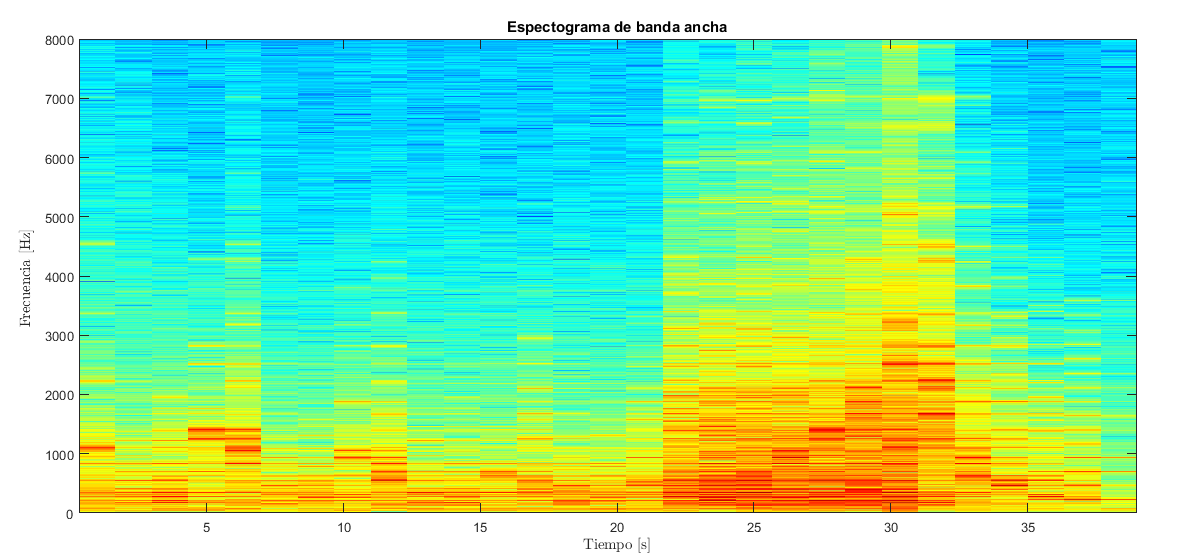
\includegraphics[scale=0.35]{1a.png}
		\caption{Espectrograma de banda ancha.}
		\label{graf:banda_ancha}
	\end{figure}

	\subsection{Banda angosta}
	
		\begin{figure}[h!]
			\centering
			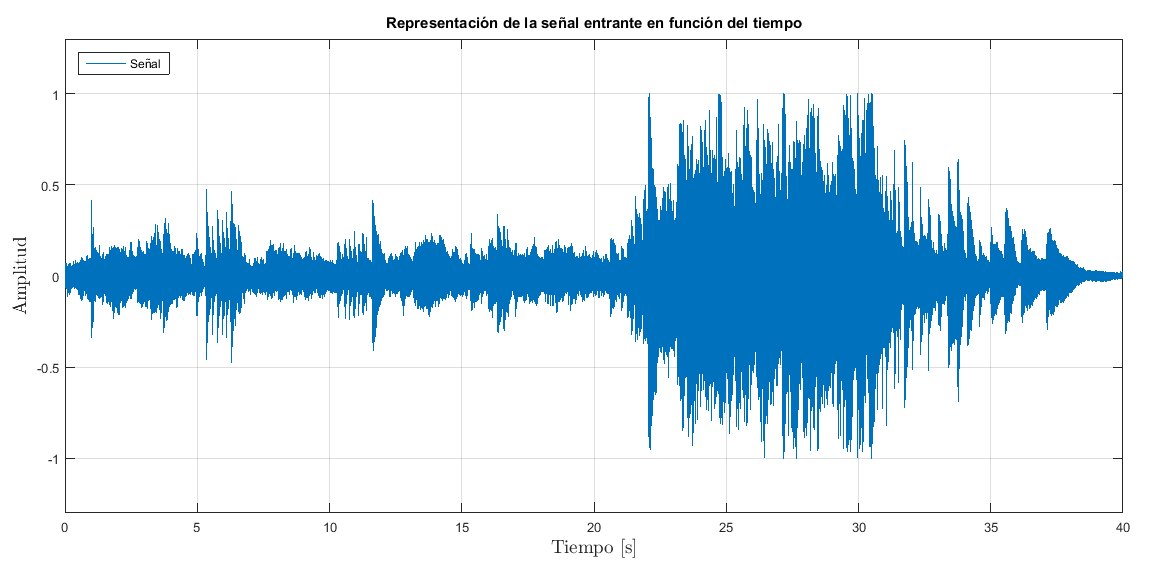
\includegraphics[scale=0.35]{Senal_temporal.png}
			\caption{Señal del archivo \texttt{audio.wav}.}
			\label{graf:senal_original}
		\end{figure}


		Suponiendo que la señal fuese un tren de pulsos, un criterio válido sería que haya 10 ventanas por pulso. A partir del gráfico de la señal de la Figura \ref{graf:senal_original}, se escoge como pulso patrón el representado en la Figura \ref{graf:pulso_patron}.

		\begin{figure}[h!]
			\centering
			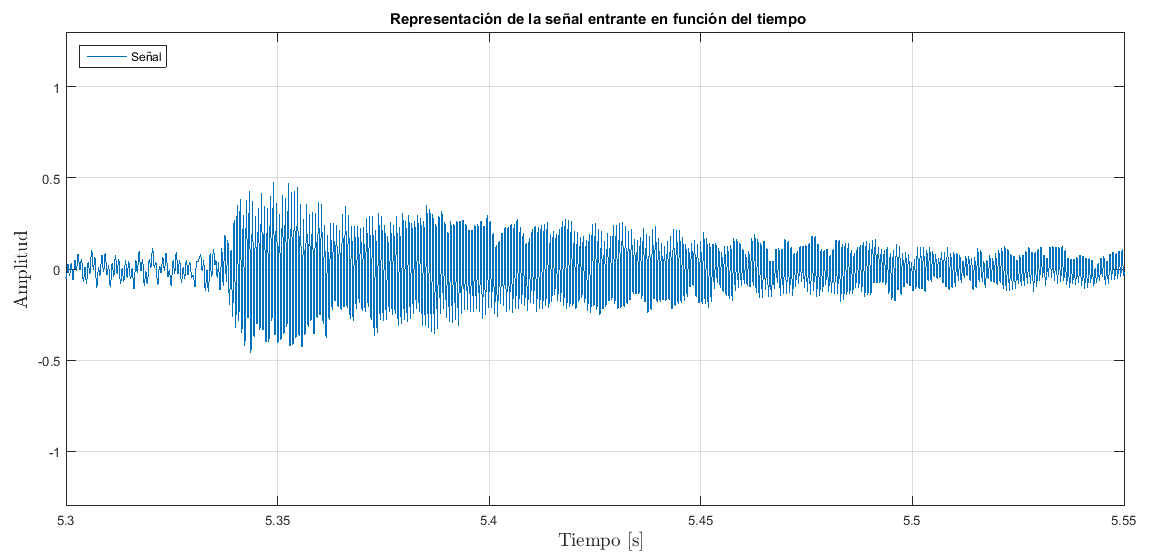
\includegraphics[scale=0.35]{Pulso_temporal.png}
			\caption{Parte de la señal original que se utiliza como patrón.}
			\label{graf:pulso_patron}
		\end{figure}

		Por lo tanto, como $t_{ventana}=\SI{.2}{\s}$:
			\begin{align*}
				10\cdot l_{ventana} &= t_{ventana} \cdot F_S\\
				l_{ventana} &= \frac{\SI{0.2}{\s} \cdot \SI{16}{\kHz}}{10}\\
				\Rightarrow l_{ventana} &= \frac{F_S}{50} = 320\\
			\end{align*}

		Con el mismo \textit{overlap} relativo y utilizando ventanas de \textit{Hamming} se obtiene el espectrograma de la Figura \ref{graf:banda_angosta}.

		\begin{figure}[h!]
			\centering
			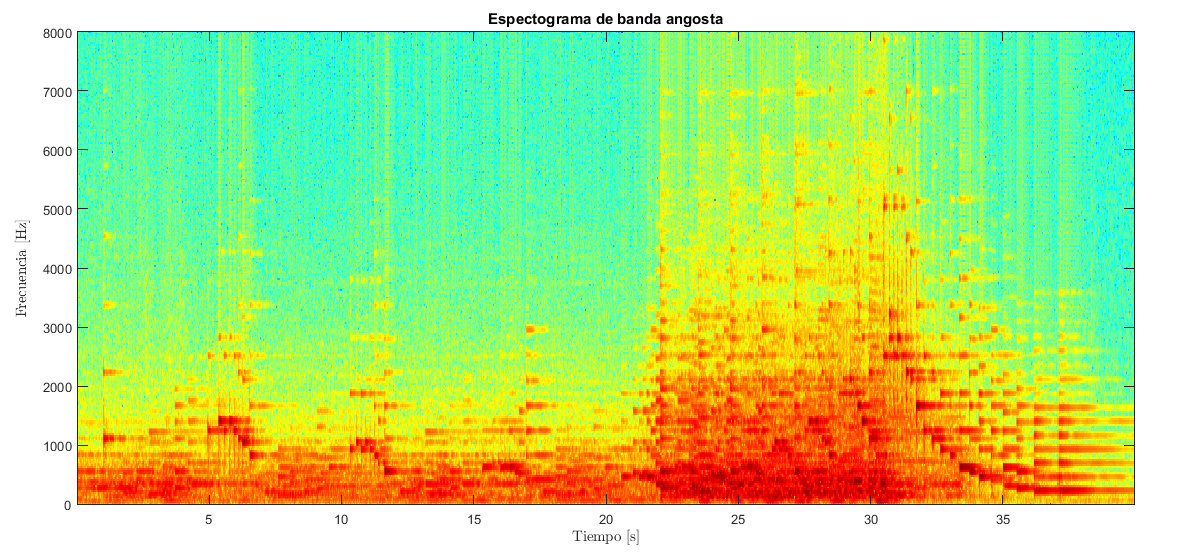
\includegraphics[scale=0.35]{1b.png}
			\caption{Espectrograma de banda angosta.}
			\label{graf:banda_angosta}
		\end{figure}
